%%
%% The first command in your LaTeX source must be the \documentclass command.
\documentclass[sigplan,screen]{acmart}
% NOTE that a single column version is required for submission and peer review. This can be done by changing the \doucmentclass[...]{acmart} in this template to
% \documentclass[manuscript,screen]{acmart}

% line breaks
%\usepackage{microtype}
%\usepackage[dvipsnames]{xcolor}

\newcommand{\karencomment}[1]{\textcolor{blue}{\textbf{\small(KAREN LEVY: #1)}}}

%%
%% \BibTeX command to typeset BibTeX logo in the docs
\AtBeginDocument{%
  \providecommand\BibTeX{{%
    \normalfont B\kern-0.5em{\scshape i\kern-0.25em b}\kern-0.8em\TeX}}}
    
\PassOptionsToPackage{numbers, sort, compress}{natbib}

%%
%% end of the preamble, start of the body of the document source.
\begin{document}%\sloppy

%%
%% The "title" command has an optional parameter,
%% allowing the author to define a "short title" to be used in page headers.
\title{Regulating Accuracy-Efficiency Trade-Offs in Distributed Machine Learning Systems}

%%
%% The "author" command and its associated commands are used to define
%% the authors and their affiliations.
%% Of note is the shared affiliation of the first two authors, and the
%% "authornote" and "authornotemark" commands
%% used to denote shared contribution to the research.
\author{A. Feder Cooper}
\affiliation{%
  \institution{Cornell University, Department of Computer Science}}
\email{afc78@cornell.edu}

\author{Karen Levy}
\affiliation{%
  \institution{Cornell University, Department of Information Science \\ \& Cornell Law School}}
 \email{karen.levy@cornell.edu}
\author{Christopher De Sa}
\affiliation{%
  \institution{Cornell University, Department of Computer Science}}
\email{cmd353@cornell.edu}
%%
%% By default, the full list of authors will be used in the page
%% headers. Often, this list is too long, and will overlap
%% other information printed in the page headers. This command allows
%% the author to define a more concise list
%% of authors' names for this purpose.
\renewcommand{\shortauthors}{Cooper, et. al.}

\begin{abstract}
In this paper we discuss the trade-off between accuracy and efficiency in distributed machine learning (ML) systems and analyze its resulting policy considerations. This trade-off is in fact quite common in multiple disciplines, including law and medicine, and it applies to a wide variety of subfields within computer science. Accuracy and efficiency trade-offs have unique implications in ML algorithms because, being probabilistic in nature, such algorithms generally exhibit error tolerance. After describing how the trade-off takes shape in real-world distributed computing systems, we show the interplay between such systems and ML algorithms, explaining in detail how accuracy and efficiency interact particularly in distributed ML systems.  We close by making specific calls to action for approaching regulatory policy for the emerging technology of real-time distributed ML systems.
\end{abstract}

%%
%% This command processes the author and affiliation and title
%% information and builds the first part of the formatted document.
\settopmatter{printfolios=true}
\maketitle

\section{Introduction} \label{sec:intro}
Engineering is defined by trade-offs---by competing goals that need to be negotiated in order to meet system design requirements. One of the central trade-offs in engineering, particularly in the field of computer science, is between \emph{accuracy} and \emph{efficiency}. More specifically, there is an inherent tension between \emph{how correct} computations are and \emph{how long} it takes to compute them.\footnote{Framing the accuracy-efficiency trade-off as a cardinal trade-off in computing importantly differs from how \citet{ohm70inefficiency} discuss efficiency. Their work calls efficiency the "cardinal virtue" of computing in order to discuss what they view as exceptional cases of inserting inefficiency into computer systems---what they term "desirable inefficiency." Instead, viewing the accuracy-efficiency \emph{trade-off} as central enables us to not refer to "inefficient" computing models as exceptional and strikes us as a more precise and generalizable statement of the issues at stake. Therefore, rather than casting particularly inefficient computing models (e.g., cryptography) as exceptional---as Ohm and Frankle do---we can conceive of them as implementing the trade-off at one end of the accuracy-efficiency spectrum (privileging accuracy).}

While this trade-off represents a general problem, it plays out in various ways across different subfields of computing. For example, in computer hardware, circuits can use approximation techniques to relax constraints on accuracy---on how they perform bitwise computations---in order to speed up performance. In image processing, varying numbers of pixels can be used to represent a given image; using fewer pixels causes a loss in accuracy of the image being represented, but also furthers space-efficiency by requiring less memory to store the image. These kinds of examples are abundant in computing. In fact, the trade-off is so ubiquitous and well-known to computer scientists that  it has even given rise to its own subfield, \emph{approximate computing}, which resides within the programming languages (PL) discipline \cite{moreau2018taxonomy, mittal2016apsurvey}. This subfield has shown that it is useful to analyze the accuracy-efficiency trade-off in the context of how \emph{error tolerant} an application is---that is, how different domains resolve the question of how much inaccuracy can be permitted, while retaining guarantees about quality and safety\cite{sampson2015thesis}.

While commonly acknowledged in some areas of computer science---perhaps to the point of mundanity---the policy implications of this trade-off remain relatively unexamined. We therefore focus this paper on analyzing its regulatory implications in the context of a particularly urgent technological domain---\emph{distributed machine learning}. We argue that the accuracy-efficiency trade-off exposes a high-level abstraction that policymakers should use to provide regulatory interventions. That is, rather than operating at one of two extremes---either solely having policymakers rely on technical experts to make high-stakes policy decisions or inundating policymakers with underlying low-level technical details---we advocate for something in between: ML systems researchers should focus on providing guarantees concerning correctness and performance, and should build associated tools to help policymakers reason about these guarantees. These tools should effectively expose the degree of uncertainty in distributed ML systems, thus facilitating lawmakers' ability to reason about and regulate the resulting risk of their deployment in high-stakes domains, such as autonomous cars and unmanned military drones.  

To make this case, we organize the remainder of this paper as follows. In Section \ref{sec:price}, we outline the general trade-off between accuracy and efficiency. We discuss how this trade-off is salient in disciplines other than computing (Section \ref{sec:common}) and then pay particular attention to the various ways it can be used to analyze different subfields of CS (Section \ref{sec:approximatecomputing}). We then provide grounding for understanding how accuracy and efficiency are in tension with each other in distributed ML systems (Section \ref{sec:sysml}). To understand the specifics of the trade-off in that setting, we first outline separately how it unfolds in ML algorithms (Section \ref{sec:ml}) and distributed computing systems (Section \ref{sec:distributedsystems}), and then bring this discussion together to clarify emergent tensions in the subset of ML systems that serve high-stakes, real-time applications (Section \ref{sec:distributedml}). Based on the overarching themes we extract in our discussion, we then close with specific calls to action regarding these systems, both in ML systems research and in policy (Section \ref{sec:policy}).

\section{The Price of Accuracy} \label{sec:price}
Gathering increasingly accurate information is a computationally expensive task that is in tension with acting efficiently. In Section \ref{sec:common} we discuss how this tension plays out in various domains outside of computing, each with their own normative concerns. We then turn our attention in Section \ref{sec:approximatecomputing} to the various accuracy-efficiency trade-offs that are inherent throughout CS. Studying this trade-off in computing generally falls under the area of \emph{approximate computing}. We use this discussion to ground our treatment in later sections of how such trade-offs play out uniquely in the context of machine learning (Section \ref{sec:ml}) and distributed machine learning systems (Section \ref{sec:sysml}).

\subsection{The Ubiquity of Accuracy-Efficiency Trade-Offs} \label{sec:common}
The trade-off at the heart of this paper is not unique to computing. It can be observed in a diverse range of disciplines, including economics, law, and medicine. In decision theory, the time-value of information is an important concept for making choices. There is a cost to gathering increasingly accurate information. Waiting to act based on information is itself an action---one that can have potentially more negative consequences than acting earlier on imperfect information. Kahneman and Tversky elaborate on this idea in their well-known cognitive psychology research concerning reasoning about uncertainty \cite{kahneman1982uncertainty}. They argue that humans use various heuristics to make decisions more efficiently, often acting on biases they have due to incomplete information. There is a tension between taking the time to gather more information and making a more informed decision---between the speed of making a decision and the quality of information used to make it.

Sunstein connects this idea directly to the potential hazards of using heuristics in legal decision-making \cite{sunstein2002heuristics}. Nevertheless, he observes that heuristics are common---and necessary---in the law to obtain a suitable balance between efficient resolution and the "best" (i.e., most accurate) adjudicative outcomes.

A number of rules in US civil and criminal procedure (e.g., speedy trial requirements, local rules imposing filing deadlines, statutes of limitations) impose time constraints for the sake of efficient case resolution; these values must be balanced against needs for thorough fact-finding and argumentation. Due process implicates both values. Some areas of law explicitly consider how to balance between them. For example, the standard for preliminary injunctive relief in the United States explicitly considers whether irreparable injury will occur because of the passage of time, if relief is not granted before the (often lengthy) full resolution of a case.

Debates about the merits of the so-called "precautionary principle" in policymaking also capture the accuracy-efficiency trade-off. The precautionary principle advises extreme caution around new innovations when there is substantial unknown risk; in operation, it effectively places the burden of proof on risk-creating actors (like chemical plants) to provide sufficient evidence that they are \emph{not} producing significant risk of harm, rather than vice versa. As with speedy trials, there is a trade-off between the time it takes to gather evidence---to highlight the risk landscape---and capturing that landscape effectively. There are legal rationales on both sides of the spectrum with regard to how this trade-off should be implemented. For example, critics of the precautionary principle could be said to favor efficiency. They find the principle to be too stringent with regard to the burden it places on accuracy; it is "literally paralyzing" in its attempts to regulate risk  \cite{sunstein2003precaution}. On the other side, others argue that the precautionary principle provides a valuable way to reason about preventing harm by shifting the burden of proof of safety to potential risk creators. They are supportive of the fact that the principle requires actors to justify the risks they create: it is worth the time cost to gather information, such that it is possible to better manage risk in the context of scientific uncertainty \cite{sachs2011precaution}.\footnote{In addition to these examples from the law, the accuracy-efficiency trade-off is salient in other aspects of governance. In particular, it plays an important role in wartime intelligence gathering. There is an inherent tension between gathering more accurate intelligence about an opponent or enemy and acting on that intelligence before it becomes stale and loses its usefulness. This is the so-called "fog of war" notion, which attempts to capture the relationship between how the uncertainty of information changes over time \cite{Clausewitz1832fog}.}

Another urgent example of the trade-off in action arises in public health---specifically, in the context of the COVID-19 pandemic and antibody tests. The World Health Organization (WHO) has recently argued that, prior to certifying COVID-19 antibodies for treatment, it is necessary to \emph{guarantee} that such antibodies confer immunity to the virus. Several medical professionals have challenged this mandate from WHO, highlighting the time-sensitive nature of taking action in the pandemic: "Demanding incontrovertible evidence may be appropriate in the rarefied world of scholarly scientific inquiry. But in the context of a raging pandemic, we simply do not have the luxury of holding decisions in abeyance until all the relevant evidence can be assembled. Failing to take action is itself an action that carries profound costs and health consequences" \cite{weinstein2020covid}. More generally, the authors claim that it is the norm for healthcare practitioners to act on incomplete information---to balance potential inaccuracies in available data with the urgency to treat serious conditions. To see this, consider an example in which a patient has a small growth on their lungs, and it is uncertain whether the growth is benign or malignant. A doctor may then be faced with the following choice: they can either perform a biopsy---a very invasive procedure---now, with the possibility that such an early stage test could yield inconclusive results; or, they can wait and see if it grows, and then biopsy it at a later stage where there can be more certain results regarding potential malignancy. The doctor is faced with a trade-off between potentially inaccurate information in the short-term and a higher certainty of accuracy (with the potential danger of not having acted quickly enough) in the longer term.
\\

\noindent These examples all concern reasoning under uncertainty, and they tease at the relationship between uncertainty and externalities of risk. Before we discuss this relationship more formally in the context of machine learning systems (Section \ref{sec:sysml}), we demonstrate how the accuracy-efficiency trade-off is widely relevant across various domains in computing.

\subsection{Trading off Accuracy and Efficiency in Computing} \label{sec:approximatecomputing}
In computing, the accuracy-efficiency trade-off is a spectrum, not a binary decision, that has implications in almost all computer science subfields (See Figure \ref{fig:tradeoff}). To capture the intuition, let us consider a familiar example---image compression to generate JPEG images. Raw images tend to be very high resolution, meaning that they contain many pixels per inch. In order to capture each pixel, such images tend to require a lot of storage space. However, it is often not necessary to use so many pixels for a high-quality image. To the human eye, a compressed version of the raw image often suffices; removing some pixels or averaging and combining the values of neighboring pixels often is not detectable. Moreover, compressing a raw image to a JPEG takes up less computer storage space and can lead to faster image processing when doing photo editing since there are fewer pixels to consider. In other words, reducing the accuracy of the image can lead to greater computational efficiencies when manipulating it.

\begin{figure}[h]
	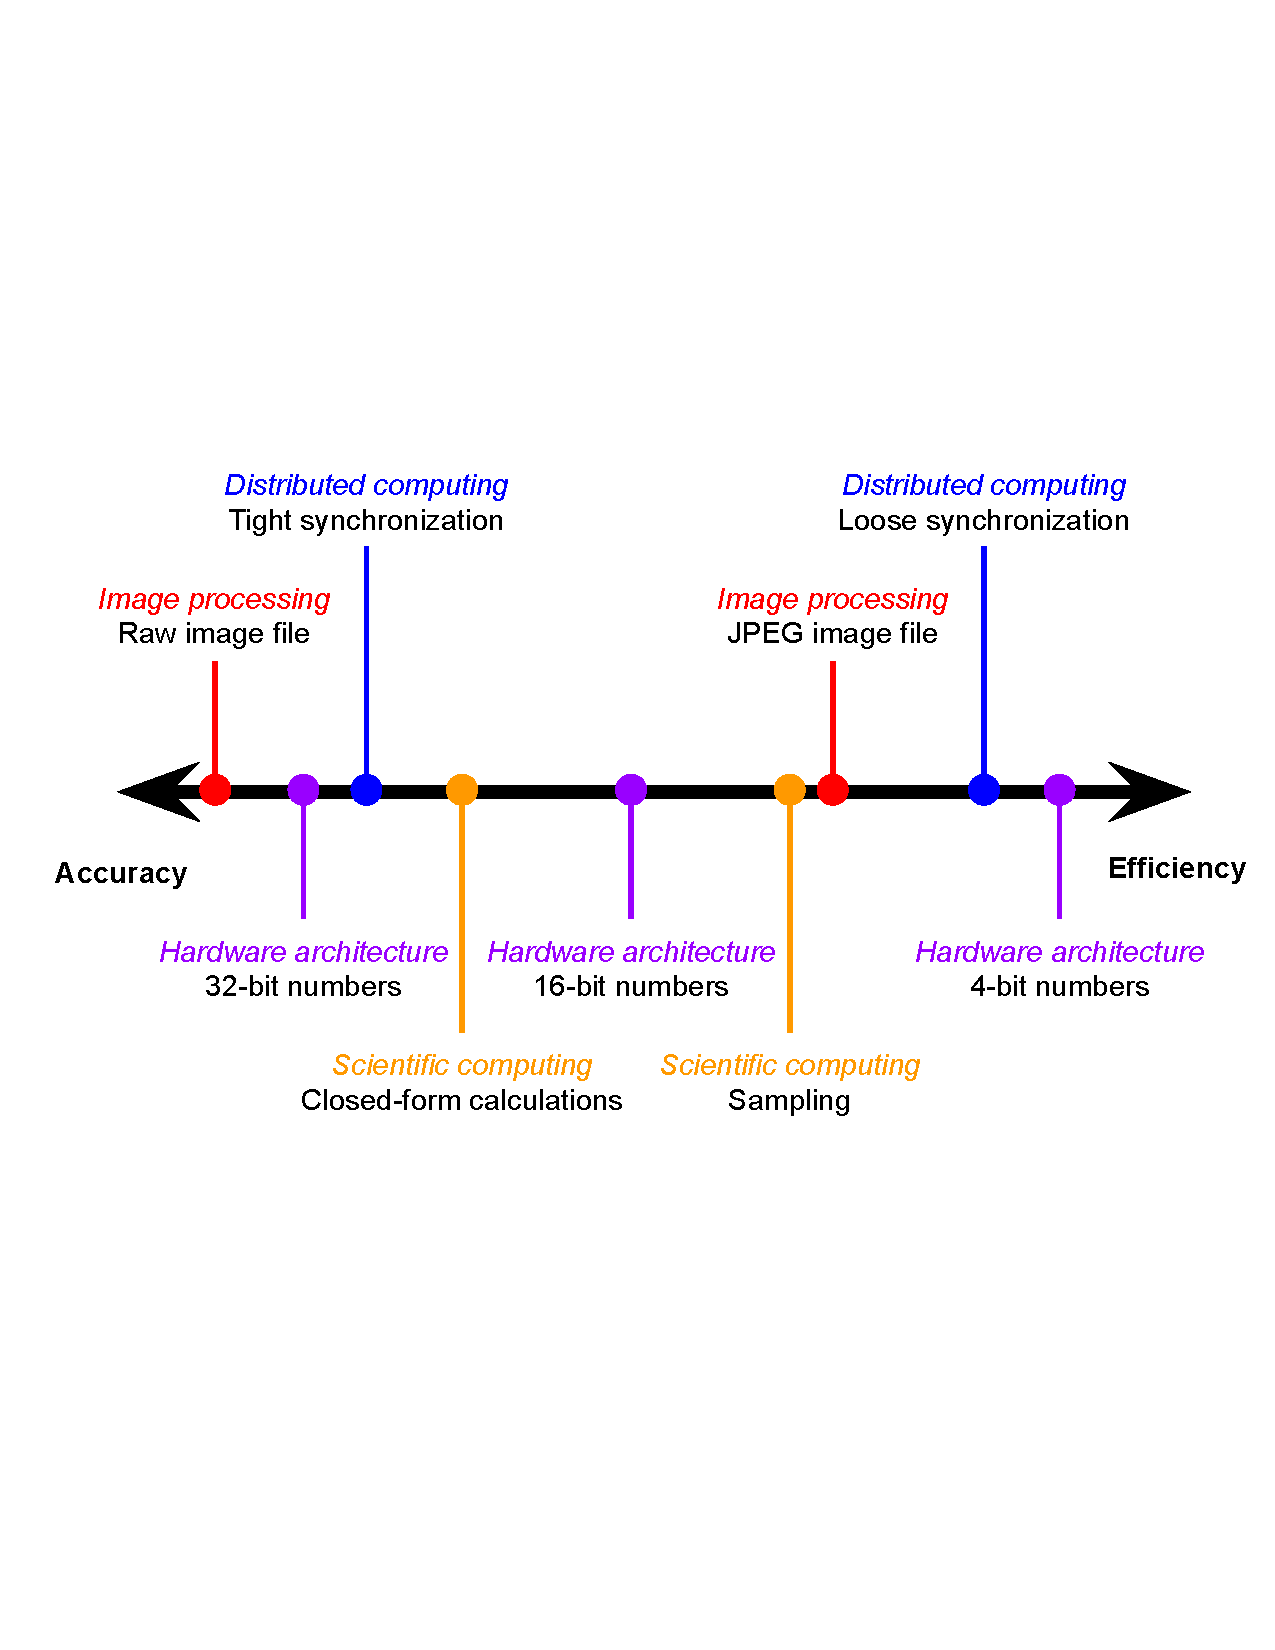
\includegraphics[width=8.25cm]{figs/accuracyefficiencytradeoff_cropped.pdf}
	\caption{Examples of implementing the accuracy-efficiency trade-off in approximate computing: \color{red}Image compression \color{black} (Section \ref{sec:approximatecomputing}), \color{violet}bit precision representing numbers \color{black}(Sections \ref{sec:approximatecomputing} \& \ref{sec:quantization}), \color{blue}distributed systems \color{black}(Section \ref{sec:distributedsystems}), and \color{orange}sampling \color{black}(Section \ref{sec:mcmc})}.
	\label{fig:tradeoff}
\end{figure}

The notion of this trade-off between accuracy and efficiency forms the basis of the field of \emph{approximate computing}. The main idea of this field is that a computer system can achieve certain performance benefits if it exerts less computational effort to compute perfectly accurate answers. In other words, it is possible to \emph{relax} accuracy in order to yield efficiency improvements \cite{moreau2018taxonomy, mittal2016apsurvey, sampson2015thesis}. As with JPEGs, relaxing the accuracy does not necessarily have negative consequences; rather, it is possible that the decreased accuracy has no observable impact for a particular application. In other words, some applications are tolerant of inaccuracy; they are error resilient.

While the term "approximate computing" is a fairly recent innovation, these ideas are as old as computers. One of the oldest examples comes from how computer hardware represents numerical values---particularly floating-point numbers, which, as opposed to integers, can have arbitrary precision; they require (potentially infinite) decimal places to express. However, computers require discretization to store numbers in binary encoding; floating-point numbers are expressed in a finite number of bits, limiting their precision and how accurately they can reflect the values of the numbers they represent \cite{moreau2018taxonomy, friedman1996bias}.

Approximate computing not only demonstrates the existence of this trade-off, but also provides ways of formally characterizing it. In turn, this characterization can enable computer scientists to leverage the "right" trade-off in different application domains. For example, formal reasoning around the trade-off can yield application-specific quality metrics. Quality can be thought of as how a program conceives of "good enough" results. Often, the quality of "good enough" cannot be guaranteed with complete certainty, but can be verified with high probability. Leaving room for uncertainty  allows for edge case behaviors, which might fall below the specified quality threshold. Quality metrics therefore capture how much an approximation is allowed to deviate from the precise version's results. Computer scientists can therefore design software that requires a certain degree of program quality with a certain (high) probability \cite{sampson2015thesis}.\footnote{A popular example of this comes from Amazon's cloud computing services (AWS). Their cloud storage service provides "11 9's" of reliability with regard to storing data objects, meaning that 99.999999999\% of the time saving such objects to the cloud occurs without error \cite{amazon2020s3}.}

\subsection{High-Stakes Application Domains} \label{sec:highimpact}
Quality metrics are particularly salient in high-impact application areas. Consider an autonomous surgical robot or autonomous car. Both application domains require both accuracy and efficiency in order to be safe and reliable, but cannot maximize both properties at the same time due to the inherent trade-off between them. Instead, in each application domain, we need to have a sense of how much error we can tolerate in order to meet certain speed demands.

The same can be said for police use of facial recognition software. For example, as described in \citet{Dietterich2018robustAI}, a study in South Wales found a false positive rate of 91.3\% in a facial recognition application that tries to match faces with outstanding arrest warrants at public events.\footnote{There have been similar findings in other cities such as Detroit \cite{lee2020detroit}.} While this application is not necessarily efficiency-sensitive---a human could, in theory, intervene to verify the accuracy of the results prior to acting---this would not necessarily be the case if such technology were integrated into police body cameras for the purpose of making in-the-moment (and potentially life-or-death) decisions. In situations of imminent danger, efficiency is crucial; for example, it is necessary to speedily identify a person-of-interest. Accuracy in this case is equally important; in heightened stress environments, mistaking someone for a person-of-interest has repeatedly proven catastrophic, particularly in the United States. Because of these competing technological goals, it is not clear exactly how approximate computing could be safe in this context, as the high stakes involved do not lend themselves to error resilience. In other high-impact legal contexts, the trade-off can potentially be reasoned about safely. Consider automated risk assessment tools \cite{starr2014risk, Chouldechova2017instruments}. Accuracy in assessing risk is critical, but is not necessarily time-sensitive. Operating on the scale of minutes, hours, or even days might suffice, particularly if such time spans entail increases in accuracy.\footnote{While this observation speaks to the trade-off between accuracy and efficiency, we do not intend for this to be taken as an endorsement for using risk assessment tools in criminal law domains. We instead apply this example narrowly to explicate accuracy-efficiency considerations, without commenting on the normative implications of what accuracy means in this context or the desirability of the use of such tools.}

\section{Accuracy-Efficiency Considerations in Machine Learning Algorithms} \label{sec:ml}
Several influential papers on artificial intelligence (AI) from the 1980s and 1990s also demonstrate the potentially high impact of appropriately dealing with accuracy-efficiency trade-offs \cite{horvitz1987constraints, boddy1994deliberation}. In particular, in a classic paper, Horvitz poses the question of how autonomous agents can effectively perform computations under tight computational resource constraints \cite{horvitz1987constraints}. He discusses how approximations or heuristics can lead to more efficient resource utilization---at the cost of potentially less-correct computation.  He frames this as a "time-precision tradeoff,"\footnote{While "precision" and "accuracy" are different, there is a relationship between them. For our purposes, it useful to think of the degree of precision as a mechanism for controlling how much accuracy is possible to achieve when performing a computation. For example, using fewer bits (i.e, low bit precision) to represent numbers can drastically effect the degree of accuracy of calculations done with those numbers, since this is effectively the same as doing computation on (potentially very highly) rounded numbers (Section \ref{sec:quantization}).} in order to indicate how there is an inherent tension between the utility of a correct computation and how fast that computation is completed, in the context of evaluating reasoning under uncertainty for autonomous agents. 

This trade-off persists beyond classical AI to contemporary work in statistical ML, as ML's probabilistic nature has important implications for the relationship between accuracy and efficiency in ML models. Trained ML models perform inference that is not always correct, often tolerating a certain degree of inaccuracy. Being resilient to errors is necessary for producing robust models. This notion of error resilience (or inaccuracy tolerance) varies for different types of ML algorithms. Regardless of particular differences, there is a general tension between \emph{correctness} and \emph{performance}. The correctness of a ML algorithm can be understood as whether or not the algorithm converged to the distribution we set out to learn, i.e., \emph{Did we learn the right model?} Its performance indicates whether convergence to the distribution---whether correct or incorrect---happened in a timely manner, i.e., \emph{How fast did we learn the model?} As with other approximate computing problems, ML can relax its demands on accuracy in order to achieve increases in efficiency. In fact, this relaxation is a requirement in many learning domains. Without it, inference computations can be so inefficient to perform that they become intractable. We describe five such cases below.

\subsection{Data Subsampling} \label{sec:subsampling}
Performance directly relates to the size of the task on which we perform learning. Intuitively, if a learning algorithm is slow on small tasks---that is, tasks with small datasets---then that algorithm will be slow, if not computationally intractable, on much larger ones. More concretely, this relationship between runtime and task size often exists due to coupling between the computation done by the learning procedure's optimization algorithm and the task's dataset size. For example, when computing the gradient needed to determine which direction the learning algorithm should step for its next iteration, it is often necessary to sum over every data point in the dataset. As we show in Figure \ref{fig:time} for the Gradient Descent (GD) algorithm, for larger datasets this summation becomes increasingly costly.

\begin{figure}[h]
	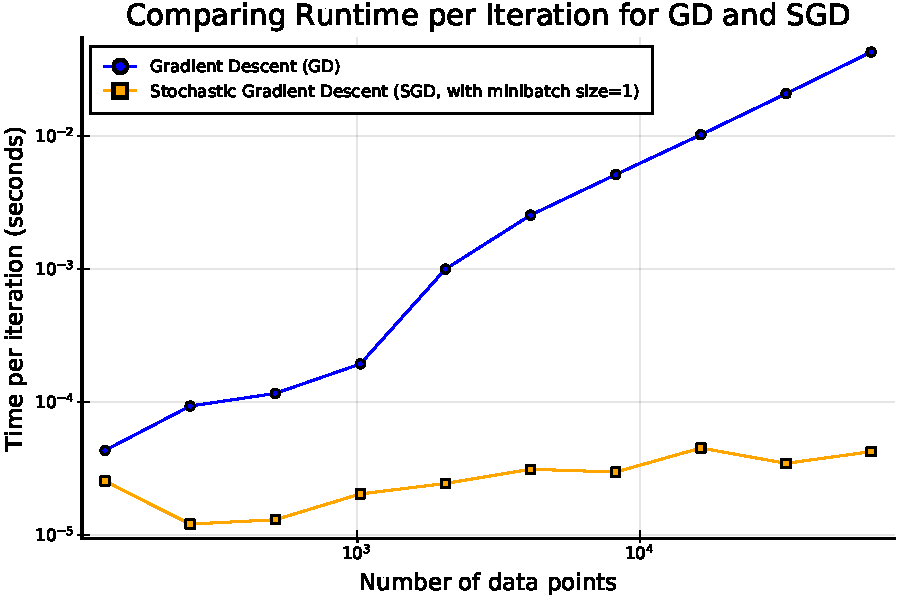
\includegraphics[width=8.25cm]{figs/timesgd.pdf}
	\caption{The runtime for GD, a full-batch method (which uses the whole dataset to compute gradients), is coupled with the size of the dataset: as the dataset size increases, so does the runtime per iteration of the algorithm. In contrast, a subsampled, minibatch method like SGD (which here uses only 1 data point to compute the gradient) is decoupled from the dataset size: it maintains a relatively constant runtime per iteration.}
	\label{fig:time}
\end{figure}

A very common approach for improving efficiency is to use a subsample or \emph{minibatch} of the dataset, rather than the whole dataset, when performing calculations. In the case of computing gradients, instead of using a "full batch" (i.e., the whole dataset) we use a randomly sampled subset of the data points, which entails spending less time on computation. Stochastic Gradient Descent (SGD) is an example of an algorithm that takes this approach. Using a minibatch can often have minimal impact on the overall accuracy of the learned model. A particular iteration of the algorithm will have less accuracy when computing the gradient (Figure \ref{fig:time}); but, when run for lots of iterations, the final result can still be statistically correct. In expectation, we can learn the same distribution as if we had been using the whole dataset in each iteration; we can often theoretically guarantee robustness \cite{Kiefer1952StochasticEO, Bottou2018sgd}.

Moreover, the decision to subsample is not all-or-nothing; it is a spectrum. It is possible to vary the minibatch size the algorithm uses. Larger minibatches---especially those that approach the size of the full dataset---require more time but are also more accurate per iteration. Conversely, smaller batch sizes make each iteration faster and more scalable to larger datasets, but in doing so sacrifice accuracy per iteration.

\subsection{Low-Precision Computation} \label{sec:quantization}
Another common approach involves using low-precision representations of the numerical values on which the computer performs computations. This method, sometimes called quantization, is similar to the idea of floating-point precision---how much accuracy the computer can capture based on how many bits it uses to represent numbers---that we discussed in Section \ref{sec:approximatecomputing}. Computing with more precise floating-point numbers is more computationally expensive; it tends to take more time (i.e., sacrifices efficiency) but can capture a more accurate range of results.

Much work in machine learning explores using low-precision numbers to achieve faster results. This work relaxes requirements on the accuracy of the trained model in order to achieve these speed-ups \cite{desa2017async, gong2014quantize, courbariaux2015binaryconnect, alistarh2017qsgd, gupta2015lowprecision,han2015deep}. As with the minibatching example in Section \ref{sec:subsampling}, this sacrifice in accuracy does not necessarily require sacrificing overall correctness if in expectation the algorithm can still theoretically guarantee learning the right distribution. There is also a spectrum at play here; similar to varying the minibatch size to tune the trade-off between accuracy and efficiency, it is possible to vary the number of bits of precision. More bits yield higher accuracy and slowdowns, while fewer bits require less time per computation and thus potentially sacrifice some correctness. Depending on a particular application's tolerance to error, this sacrifice in accuracy can be worth the speed-ups it creates \cite{desa2018halp}.

\subsection{Resource-Constrained Machine Learning} \label{sec:resources}
The prior examples discuss the cost of running computations. Specifically, they discuss how differently-sized batches of data (Section \ref{sec:subsampling}) and how differing degrees of numerical precision (Section \ref{sec:quantization}) directly impact how long it takes a computer to execute a computation. Even though these examples concern a computer's behavior, we have not yet considered how hardware specifications of the computer running the algorithm might impact that behavior. Surely this is important, as different computers have different computing capabilities due to varying hardware; a NASA supercomputer has more computational resources than a personal laptop.

Recent years have seen an increase in the variety of computational devices available and a corresponding increase in the variety of computations we wish to run on them. For example, Internet of Things (IoT) devices and sensors, such as Google Home or Amazon Echo, perform inference. They serve up answers to spoken language questions; however, they also have limited on-board capabilities to perform computations locally. These limitations take several forms. For example, such devices might not have a lot of power to process data quickly or might lack storage capacity for large amounts of data.

Often, these devices can communicate with more sophisticated computers over the Internet, offloading computation or storage to those computers. However, this communication exposes another trade-off between accuracy and efficiency; it takes time to send the data to a remote computer, perform some computation, and then return a response to the device \cite{birman2019cloud}. That computation may be more accurate, but achieving that accuracy comes with a cost in speed. Conversely, doing the computation locally on the device would be faster; however, due to the device's more limited computational resources, it will not necessarily be very accurate.

Prior work considers how computer vision models can be learned and stored on a mobile device like a smartphone.\footnote{Aside from being faster, there are several reasons why such local computation and storage might be desirable for a mobile application, as opposed to communicating with and offloading these requirements to more powerful remote computers. Notably, local computation can ensure privacy, as the learned model and collected data never leave the mobile device.} For such resource-constrained devices, different applications have different needs in terms of how to trade-off between how accurately and how quickly a computation is performed. Some prior work has explored these application-specific needs, providing an interface for flexibly implementing different points along the accuracy-efficiency trade-off spectrum. For example, MobileNets contains manually-tunable parameters that allow the model developer to strike the right balance for particular learning problems \cite{howard2017mobilenets}. Depending on the application domain, the developer can tune a larger model that uses more resources (i.e., a model that is slower but more accurate) or one that is smaller and uses fewer resources (i.e., a model that is faster but less accurate).

\subsection{Markov chain Monte Carlo Sampling} \label{sec:mcmc}
We now delve into a slightly more sophisticated example. We consider a branch of ML that has recently proven particularly useful in the probabilistic modeling of data for Bayesian inference: Markov chain Monte Carlo (MCMC) sampling. To understand MCMC, it's first important to have an intuition regarding how sampling works. We will explain sampling by way of a simple, familiar example: flipping a coin.

When flipping a normal coin, it can either result in "heads" or "tails," with a 50\% chance for yielding each. Let us consider that it is possible for a coin to be biased---that the coin is weighted in such a way that, when flipped, it yields heads 60\% of the time. In order to figure out how biased the coin is---the probability it yields heads---we flip the coin repeatedly to generate samples of the coin's behavior and record the results. That is, we flip the coin for multiple trials, and after each trial we update the estimated probability that the coin yields a heads result. We can view this updating probability as the information we are learning---we are generating a model of the coin's behavior, which we store as the probability of flipping heads. When we begin flipping the coin, there are not many generated samples. As a result, as shown in Figure \ref{fig:coinflip} our estimation of the probability of heads might change a lot; it can update fairly erratically. Over time, as we generate more samples, the probability estimate becomes more stable. We converge to a probability that does not change very much, giving us a fairly good estimate of the coin's bias.  

\begin{figure}[h]
	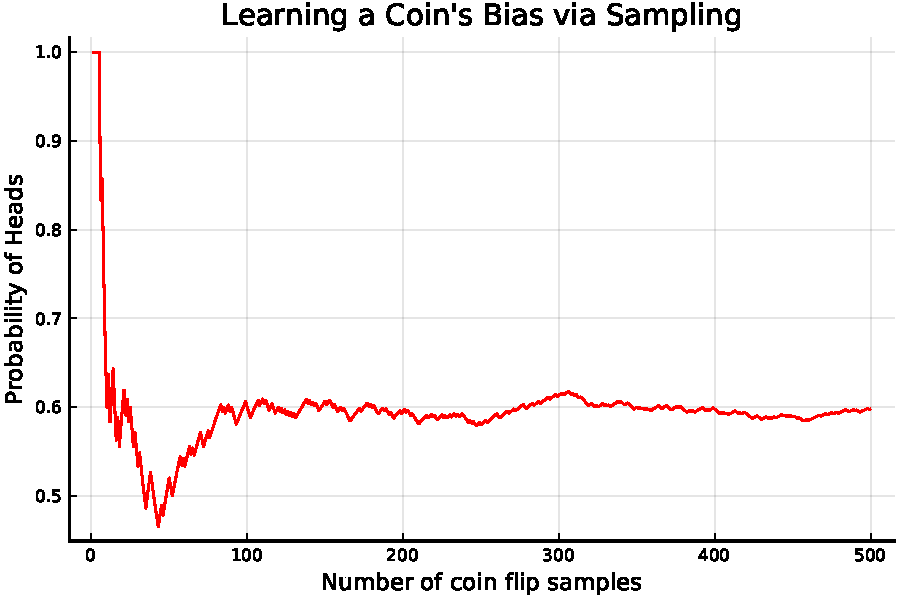
\includegraphics[width=8cm]{figs/flip.pdf}
	\caption{Generating samples of a coin flip to determining a coin's bias (in this case, 60\% heads).}
	\label{fig:coinflip}
\end{figure}

MCMC can be thought of as a more complicated instantiation of a sampling method like this. Instead of learning the probability of a biased coin, we are trying to learn the parameters of a desired probability distribution. To do this, we construct a Markov chain, from which we iteratively produce samples. Similar to updating the estimated bias of the coin after each sampling iteration, in each iteration of MCMC we update our estimation of the distribution parameters. Eventually, the values of the parameters become stable; we converge to an equilibrium in which the samples we continue to draw reflect the desired distribution \cite{brooks2011handbook}.

While this technique is very powerful for accurately performing Bayesian inference, it comes with significant performance drawbacks. In particular, when the learning problem's dataset is large, the performance of an MCMC algorithm often suffers. Just as in Section \ref{sec:subsampling}, efficiency and scalability become limited due to computations that require summing over every data point in the dataset; performance is therefore (loosely speaking) inversely proportional to the size of the dataset. Additionally, just as before, we can lessen these limitations by introducing subsampling---by using a randomly selected minibatch of data instead of the whole dataset. However, as we have seen with the accuracy-efficiency trade-off, there is no free lunch; the speed-ups from minibatching can introduce inaccuracy. More specifically, we can lose the guarantee of converging to the correct desired distribution, which can yield potentially disastrous inference results \cite{zhang2020tunamh}. Instead of yielding \emph{exact} results, the randomness from using minibatches can introduce bias that entails \emph{inexact} results.

Prior work makes the case that inexactness can be worth its performance gains---that it is better to be faster even if there is a risk of losing accuracy, since it can enable scaling up MCMC to big data inference problems. As a result, there is a rich scholarly literature concerning inexact minibatch MCMC methods  \cite{chen2014stochastic,korattikara2014austerity, seita2016efficient}. However, in practice, data science practitioners often do not use inexact methods; for reliability, they find that it is better to be slow and correct than fast and wrong. Recent work therefore attempts to construct new minibatch MCMC methods that retain exactness---methods that have theoretical guarantees regarding accuracy while also incorporating certain tricks and statistical insights that enable preserving some of the speed-ups minibatching provides \cite{maclaurin2015firefly, zhang2019poisson, zhang2020amagold, cornish2019scalable, zhang2020tunamh}. In other words, these exact methods lean toward the accuracy side of the accuracy-efficiency trade-off; they guarantee converging to the correct, desired distribution, but to do so they sacrifice speed in relation to their inexact counterparts, particularly on some types of learning tasks.

\subsection{Asynchronous ML} \label{sec:async}
Finally, we examine the trade-off in machine learning in \emph{asynchronous} settings. The examples we have discussed so far are \emph{synchronous}: there is one computer process\footnote{A computer can run multiple \emph{processes} at once. Each process is an instance of a running program---this is why one can run both an Internet browser and a text editor at the same time. In other words, processes allow for parallel tasks to run on one computer \cite{ArpaciDusseau2018os}.} that does all of the computation, one step at a time. In contrast, it is possible to run computations \emph{asynchronously}, in which different computer processes or threads\footnote{A thread is a further mechanism for parallelization on a computer, which operates at the level of a process. That is, a process can have multiple threads running at the same time. For example, this is what allows a text editor (which is running in a process) to simultaneously enable displaying both typing and syntax-error highlighting in real-time. Each of these functions happens in its own thread of computation.} perform computations side-by-side. This facilitates dividing computationally intensive tasks into parts, such that different portions can happen in parallel and then can be combined to compute the final result.

In other words, the parallelization from asynchrony can lead to speed-ups in ML since multiple parts of the learning problem can be computed at once. However, depending on how the parallel results are combined, it can also lead to decreases in accuracy. That is, if different processes end up working on the overlapping parts of the overarching computation, the process that finishes its computation second can overwrite the value computed by the one that finished first, causing inaccuracies in the results \cite{desa2017async, alistarh2018convergence, lian2017asynchronous, Niu2011hogwild}. This can be avoided by forcing the different processes to coordinate their updates, such that they do not overwrite each other. However, such coordination takes time; it enables more accuracy, but decreases efficiency. In some cases, this overwriting is worth the speed-ups it enables; it is still possible to compute good quality learning estimates \cite{desa2016gibbs, daskalakis2018gibbs}.\footnote{Asynchrony is complementary to other examples in this section. For example, it can be used in combination with minibatching, low-precision, and in MCMC to implement other types of accuracy-efficiency trade-offs.}
\\

\noindent So far, our discussion does not take into consideration how the accuracy-efficiency trade-off behaves for ML in real-world, deployed systems---systems that often consist of multiple computers that communicate and work together to solve large, complex problems. Such systems often communicate asynchronously: instead of one computer doing multiple sub-computations at the same time (Section \ref{sec:async}), there are multiple computers operating in parallel on the same problem. In the next section, we discuss how such real-world distributed ML systems raise unique concerns with regard to accuracy and efficiency.

\section{Making Sense of Additional Trade-Offs in Real-World ML Systems} \label{sec:sysml}
Our overarching aim is to understand the particular tensions between accuracy and efficiency for \emph{distributed machine learning systems}, and how these tensions differ from those we discussed regarding machine learning algorithms in Section \ref{sec:ml}. To make these distinctions clear, we first clarify some key ideas from distributed computing in Section \ref{sec:distributedsystems}.\footnote{We touch on this topic only briefly, since our main focus is the behavior of such systems in the context of \emph{machine learning} For more detailed treatment, see \citet{cooper2019isp} and \citet{cooper2020law}.} From this basis, we can then layer on more complexity in Section \ref{sec:distributedml}. We weave in our understanding of the accuracy-efficiency trade-off for ML algorithms from Section \ref{sec:ml} and observe how the different tensions interact with each other. Considered together, we demonstrate how machine learning and distributed systems trade-offs present especially challenging problems for real-time, high-impact systems like autonomous vehicles. These real-time domains inform our policy discussion in Section \ref{sec:policy}.

\subsection{Accuracy and Efficiency in Distributed Systems} \label{sec:distributedsystems}
In contrast with a single, solitary computer, a \emph{distributed system} is a network of computers that communicate with each other. Via this communication, the computers can work together to solve problems. Each computer in the network has its own data and performs its own computations, and it shares data and computation results with other computers in the network when necessary. For example, if a computer needs data from another computer in order to execute a computation, it can request the data from that computer.

Because the computers are in distributed locations and need to communicate, there are important considerations with regard to how efficiently information can be shared between them. That is, when a computer contacts another in the system to request its data, it takes time to complete the request and receive the data---in direct opposition to efficiency. There are also issues of accuracy between computers in the system. Each computer has its own data---its own snapshot of what it knows to be the state of the overarching system. However, that information is not complete; it is just a subset and can possibly contradict the information that other computers in the system have. Simply put, the computers can be inconsistent with each other.

In other words, in distributed systems we can frame the trade-off between accuracy and efficiency as a tension between \emph{consistency} and \emph{latency}---the speed with which the system updates. There is a trade-off between all of the computers in the system having the same understanding of the data in the system and the time it takes to propagate that understanding throughout the system \cite{Abadi2012tradeoff, Brewer12computer}. Due to this trade-off, in distributed systems that update their data frequently it is actually quite difficult to quickly build a consistent, holistic understanding of the environment across different computers in the network. This is because consistency is a moving target; each computer processes information locally faster than it can share it with the entire network. Given that it takes time to communicate, it is hard for computers to stay completely up to date with each other.

Nevertheless, for the sake of efficiency, individual computers in the system often need to make decisions in the presence of inconsistency. Otherwise, because of the tension between consistency and latency, waiting for complete consistency across computers before a computer could make local changes would bring the entire system to a standstill. Instead, particular distributed system implementations need to answer the question of how much inconsistency and slowness they can each tolerate, which is often application-dependent.

To understand this spectrum, we will consider a few examples of distributed systems that implement the trade-off differently \cite{DeCandia2007dynamo, Herlihy1990apologizing}. First, consider a social media website, which has computers hosting its data distributed all over the world. A user visiting the site from a personal device tends to access the geographically closest computer server hosting the site; different users across the world therefore access different computer servers. Such a system favors efficiency (i.e., low latency) over the different computer servers being consistent with each other. It is more important to return the website to each user quickly than it is to make sure that every user is accessing the website with exactly the same data. This is why on some social media sites it is possible to see out-of-order comments on a feed; the site is making a best effort to resolve its current state, which entails aggregating information from across the system. It attempts to build a consistent picture, but limits how much time it spends doing so---sacrificing consistency---so that it can remain fast  \cite{DeCandia2007dynamo, Lu2015Existential, Vogels2009eventualconsistency}. The system implements this choice via its communication strategy. Rather than contacting every computer in the system to construct a coordinated, consistent picture (which would take a lot of time) a particular computer only communicates with a subset. It trades off the accuracy it would get from communicating with every computer for the efficiency of communicating with fewer computers \cite{krishnamurthy2002tunable, hellerstein2019calm}.

In contrast to an efficiency-favoring social media site, blockchain technology is a distributed system for storing a transaction ledger that favors consistency at the cost of being slow\cite{nakamoto2012bitcoin}. In short, it is a distributed system where each computer has its own copy of the entire ledger. When a computer wants to add a transaction to the system, it has to broadcast that information to every computer in the network. All of the computers need to agree on the validity of a transaction before it can be included. As a result, the system proceeds in lockstep, only when there is coordinated agreement.\footnote{This is a tremendous oversimplification for brevity, since the point of introducing this example is to explain trade-offs between accuracy and efficiency. A more detailed treatment appears in \citet{narayanan2016bitcoin}.}

These different implementation choices reflect different design goals. The cloud was designed for e-commerce applications, in which supplying (even potentially inaccurate) responses quickly to the user is critical for user engagement \cite{bailis2012pbs, brutlag2009speedmatters}. For blockchain systems, consistency is paramount; it is crucial that all of the computers agree with each other about the state of the ledger, because it is this agreement that facilitates its reliability as a transaction record.

While these two examples seem to imply that there is an all-or-nothing choice in the trade-off between consistency and latency in distributed systems, this is not the case. Like accuracy and efficiency more generally in approximate computing (Section \ref{sec:approximatecomputing}), the trade-off between consistency and latency is a spectrum \cite{Abadi2012tradeoff, Yu2000conits}. It is possible to quantify consistency and to measure and monitor its maintenance throughout a distributed system  \cite{Lu2015Existential, Shang2018rushmon}. Developers can reason about the degree of inconsistency their particular system can tolerate safely, and can detect and tune the system's implementation accordingly to also enforce an upper bound on latency \cite{Golab2011funandprofit,barbara1990controlledinconsistency, du1989quasi, ramaritham1995eserializability, TorresRojas1999TimedCF, Yu2000numerical}.

\subsection{Bringing it All Together: Trade-Offs in Distributed Machine Learning Systems} \label{sec:distributedml}
Given this background on how accuracy and efficiency are in tension with each other in distributed systems in general (Section \ref{sec:distributedsystems}) and our earlier discussion of accuracy-efficiency trade-offs in ML (Section \ref{sec:ml}), we can now specifically consider real-time (i.e., latency-critical) distributed ML systems. As an example, consider a distributed system of autonomous vehicles. Numerous vehicles are potentially networked together and with other devices, such as smart traffic lights. Moreover, while each vehicle moves throughout the environment with its own local notion of the state of the environment, information that other vehicles possess could also prove useful. For example, if an accident is up ahead, a vehicle closer to the crash can communicate that information to the vehicles behind it, which in turn can apply pressure to their brakes and potentially prevent a pile-up.

In such real-time transportation domains, accuracy and efficiency\footnote{For consistency with the main framing of the trade-off between accuracy and efficiency in this paper, we will use this language, instead of consistency and latency, going forward. However, as noted in Section \ref{sec:distributedsystems}, consistency and latency can be viewed as cases of accuracy and efficiency, respectively.} are both critical. Some ML inference applications may be error tolerant, but in high-stakes domains this may not always be the case; it is unclear how much inaccuracy will be tolerable while still ensuring safety.\footnote{For more on the normative values at play in such situations, please refer to \citet{cooper2020law}.} The way such systems will need to treat efficiency is similar. They will need to make decisions quickly and, much like the non-computing examples in Section \ref{sec:common}, there is an inherent trade-off between waiting to make a completely informed decision and making a decision fast enough for it to be useful \cite{Abadi2012tradeoff, Brewer12computer}. What is different here is the degree of efficiency needed---in some cases, inference decisions will be necessary at subsecond speeds.

In short, it is not entirely clear what the right design goal is for real-time systems like autonomous vehicles and how the trade-off should be implemented for them \cite{Dietterich2018robustAI}. Given the dynamic nature of the environment, the particular trade-off implementation may depend on context. Some environments will be more efficiency-critical: it would be catastrophic for a car to take an extra half-second to be certain that there is a pedestrian directly in front of it. In other cases, having an accurate sense of the environment may be more important than allowing the cars to operate quickly. For example, when detecting a deep pothole up ahead, it could be safer for a car to slow down to decide its course of action---to accurately determine if the hole is shallow enough for the car to continue on its course or if the hole is deep enough to warrant veering off the road to avoid it.

Distributed ML systems raise different accuracy-efficiency questions than either distributed systems that do not involve ML, or ML systems that are not distributed. With regard to the former, the kinds of coordination and consistency issues that distributed systems can tolerate while maintaining correctness are different in nature than what newer ML systems can tolerate (particularly around issues like numerical error and staleness) \cite{bailis2012pbs, DeCandia2007dynamo,Yu2000numerical}. With regard to the latter, as we saw in Section \ref{sec:ml}, since ML models (necessarily imperfectly) approximate representations of the world, it is possible for ML models to operate on data that are not completely accurate and still yield results that are correct enough---that fall within the same bounds of imperfection that we deem tolerable when operating on accurate data. We can extend such data inaccuracies beyond things like subsampling to include data staleness inherent in asynchronous distributed settings. Allowing for such staleness comes with the benefit of increasing efficiency, as the system would not need to wait to synchronize---to completely resolve staleness issues before proceeding with its computation. Similar to the single computer case, their overall output still \emph{can be} correct even when operating on numerically imprecise or stale data in a distributed setting; however, existing work in this field does not necessarily guarantee such output \emph{must be} correct \cite{alistarh2018convergence,dutta2018slow, gong2014quantize, lian2017asynchronous, Niu2011hogwild, desa2015taming, zhang2015sgdstaleness}.

Instead, prior work has examined this phenomenon at a high level by looking at the correctness and the performance of end-to-end ML systems, rather than directly evaluating the underlying accuracy-efficiency trade-off. This work focuses on empirical results for tuning the staleness of the underlying data storage layer. Tuning has generally either been manual---curated to the particular problem domain---or absent, leaving the user to pick from a few predefined settings that enforce high accuracy, ignore accuracy altogether for efficiency, or attempt some middle-ground, "in-between" approach \cite{Abadi2016tf, ho2013SSPParameterServer, Li2014parameterserver, kosaian2019paritymodels, pan2016cyclades}. Attempts at more flexible trade-offs have entailed very domain- or algorithm- specific solutions \cite{Lloyd2011COP, pan2013occ, Wei2015managed}.

While it is possible to implement any of these different points in the trade-off, current large-scale systems for distributed learning and inference tend to opt for efficiency. They focus on minimizing communication between computers in the system in order to be efficient enough to scale to larger problems. Some of these systems can achieve orders of magnitude in performance improvements by dropping updates without simultaneously destroying correctness \cite{Niu2011hogwild, tsitsiklis1986stochastic}; however, it is not clear these approaches will work for real-time distributed ML systems that are safety-critical, such as autonomous vehicles. It will not always be feasible for these systems to lose updates. Existing approaches to mitigate such losses in ML systems involve increasing communication between computers in the system. However, this then impacts the other side of the accuracy-efficiency trade-off, leading to inefficiencies from bottlenecks in coordination between computers.\footnote{This problem is similar to what exists in weakly consistent storage systems, which have side-stepped this issue by using semantic information to coordinate "only when necessary" \cite{Badrinath1992beyondcommutativity, DiPippo1997semanticcc, Herman2016typeaware, molina1983semantic, weihl1988commutativity}.}

\section{A Call to Action: Enabling the Regulation of the Accuracy-Efficiency Trade-Off} \label{sec:policy}
We have taken considerable space to clarify a variety of accuracy-efficiency trade-offs---from how they generally impact the field of computing to how they describe the range of possible behaviors for distributed machine learning systems.

More specifically, it is necessary and urgent to expose the accuracy-efficiency trade-off because it is a potential lever for regulation. Though various manifestations of the trade-off are well-acknowledged in technical communities, they have not, to date, been legible to policymakers. We argue that policymakers must understand the implications of the accuracy-efficiency trade-off in order to responsibly regulate emerging technologies---that it is necessary and urgent to expose the trade-off as a potential lever for regulation. 

As we have documented in Sections \ref{sec:approximatecomputing}-\ref{sec:distributedml}, this trade-off is not binary; it is a spectrum and can be treated like a tunable dial set appropriately to the context. Our hope is that exposing this dial will provide a certain degree of technical transparency to lawmakers, such that high-stakes systems do not get deployed without sufficient public oversight \cite{cooper2020law, cooper2019isp}. Contemporary policy debates about high-stakes, time-sensitive machine learning applications---in domains like policing, warfare, and public health---often involve concerns about what degree of accuracy we ought to demand from such systems. These concerns often arise in the course of attempting to minimize disparate outcomes across groups (e.g., differential accuracy rates for face recognition along dimensions of race and gender \cite{buolamwini2018gender}). But debates about the harms of inaccuracy are incomplete if they fail to acknowledge and reckon with the technical trade-off between accuracy and efficiency. Accuracy may necessarily be limited when speed is essential, and as we have seen, the speed of decision-making can implicate important public values as well \cite{cooper2020law}. Informed policy debate about machine learning must pay attention to the limits imposed by this trade-off.

Beyond exposing this trade-off, we also propose a twofold call to action. The first portion of this call is for computer scientists. While our work here exposes the trade-off between accuracy and efficiency and how to engage with it---to build systems that can prioritize application-dependent balances between the two---it also indicates gaps in existing approaches in real-time ML systems. These gaps imply that existing systems will likely not suffice for high-stakes, emerging applications such as autonomous vehicles. In particular, in Section \ref{sec:distributedml} we explain the importance of needing to make the accuracy-efficiency trade-off transparent in a system's implementation; a system's ability to be assessed with regard to this trade-off should be considered as important as every other technical feature. A potential future research direction could mathematically formalize the semantics of the trade-off in ML systems. This could enable building tools to optimally tune the trade-off between consistency and latency for different classes of distributed ML algorithms, balancing their individual accuracy and efficiency needs.

Such tools would also provide policymakers with insight into how certain implementation decisions impact overall system behavior. This is crucial because, as we have shown throughout this paper, low-level technical decisions are not trivial; they should not be dismissed as "just implementation details" left up to the whims of engineers without public oversight. To be clear, we are not claiming that policymakers need to understand the full extent of low-level technical details to provide this oversight. Rather, we are suggesting that surfacing the higher-level trade-offs that lower-level decisions entail clarifies valid sites for potential policy intervention \cite{cooper2020law, mulligan2018governance, jasanoff2016ethics}. One can then think of such trade-offs as the right layer of abstraction with which policymakers can engage. At this level, policymakers can reason about the normative values and policy goals implicated by the trade-off in different domains~\cite{cooper2020law, flanagan2008values, friedman2019values}. The case of the accuracy-efficiency trade-off, for example, can be used to clarify how lower-level engineering decisions relate to notions of safety and quality \cite{sampson2015thesis}.

It is this reasoning that informs the second part of our call to action: policymakers should view the accuracy-efficiency trade-off as a regulable decision point at which they can meaningfully intervene. They can use these trade-offs to assess the expected behavior of real-time ML systems. As a result, we can fairly pose to policymakers questions like the following: At what point should we deem information of sufficiently high quality to justify the execution of potentially high-impact decisions by technical systems? When is it safe for a system to spend more time computing inference outcomes, particularly when more efficient heuristics do not sufficiently remove uncertainty from automated decision-making?

In other words, by giving policymakers the tools to reason about these higher-level trade-offs, we are able to take a step toward closing what Jasanoff terms the "responsibility gap." That is, policymakers will have a more sufficient understanding of technology and will be better equipped to gauge the range of possibilities for its governance. This way, when technological failures occur, rather than viewing them simply as "unintended consequences" or "normal accidents" \cite{perrow1999risk}, policymakers can more actively participate in the evaluation of how uncertainty in probabilistic, automated decision systems contributes to the construction of risk \cite{jasanoff2016ethics, hilgartner1992risk}.

\section{Conclusion} \label{conclusion}
This two-pronged call to action highlights the relationship between uncertainty and risk in distributed machine learning systems. By providing a mechanism to reason about the accuracy-efficiency trade-off, computer scientists expose a particular kind of decisional uncertainty that depends on time \cite{horvitz1987constraints, boddy1994deliberation}. Clarifying this uncertainty does not, however, identify specific risks that these automated decisions bring about. Given the uncertainties involved, it is up to regulators to frame potential risks and to identify the normative, domain-specific values at play \cite{jasanoff2016ethics}. That is, while computer scientists can reason about how much error is tolerable due to the accuracy-efficiency trade-off (Section \ref{sec:approximatecomputing}), we contend that policymakers and regulators need to determine how much of the resulting risk is tolerable. 

In select cases, in which it is possible to deem the amount of predetermined risk to be intolerable, policymakers could disallow particular technical systems from widespread deployment \cite{sachs2011precaution, Dietterich2018robustAI, perrow1999risk}. However, in most cases, it may not be possible to preemptively fully analyze the risk landscape~\cite{sunstein2003precaution, smith2015opportunism}. Instead, this is where exposing the trade-off between accuracy and efficiency can lead to accountability after-the-fact \cite{backes2009csar, Haeberlen2007peerreview, Lampson2004security}. In other words, when deployed in the wild for long enough, due to their complexity real-time, high-stakes ML systems are likely to incur harm \cite{perrow1999risk, vaughan1996challenger, Nissenbaum1996accountability}. Given that this is unavoidable, it is important to build tools like those we call for in Section \ref{sec:policy}. This way, it will be possible to determine if a system has deviated further than expected from its normal (what we consider to be acceptable) behavior \cite{sampson2015thesis}---cases in which policymakers and regulators can hold the appropriate stakeholders to account.

\begin{acks}
This work was made possible by generous funding from Adrian Sampson and the John D. and Catherine T. MacArthur Foundation. We would like to thank Jaime Ashander, Ken Birman, Em Feder Cooper, Thomas G. Dietterich, James Grimmelmann, Ido Kilovaty, Kristian Lum, Alan Mackworth, Helen Nissenbaum, Alec Pollak, and Matthew Sun for their comments and suggestions on various versions of this work---with particular appreciation given to Harry Auster for his incisive feedback.
\end{acks}

\section*{Code}
The code used to generate Figures \ref{fig:time} and \ref{fig:coinflip} can be found at \url{https://github.com/pasta41/lml-2020}.

%%
%% The next two lines define the bibliography style to be used, and
%% the bibliography file.
\bibliographystyle{ACM-Reference-Format}
\bibliography{sample-base}

\end{document}
\endinput




